\documentclass[12pt, openright, oneside, a4paper, brazil]{abntex2}
\usepackage{lmodern}
\usepackage[T1]{fontenc}		% Selecao de codigos de fonte.
\usepackage[utf8]{inputenc}
\usepackage{lastpage}
\usepackage{amsmath}
\usepackage{indentfirst}
\usepackage{color}				% Controle das c ores
\usepackage{graphicx}			% Inclusão de gráficos
\usepackage{microtype} 			% para melhorias de justificação
\usepackage[brazilian,hyperpageref]{backref}	 % Paginas com as citações na bibl
\usepackage[alf]{abntex2cite}	% Citações padrão ABNT
\usepackage{trabalho}	% Citações padrão ABNT
\usepackage{lipsum}				% para geração de dummy text
% ---

% ---
% Pacotes de citações
% ---

% --- 
% CONFIGURAÇÕES DE PACOTES
\renewcommand{\backrefpagesname}{Citado na(s) página(s):~}
\renewcommand{\backref}{}
\renewcommand*{\backrefalt}[4]{
	\ifcase #1 %
		Nenhuma citação no texto.%
	\or
		Citado na página #2.%
	\else
		Citado #1 vezes nas páginas #2.%
	\fi}%

\titulo{TÍTULO DO TRABALHO}
\autor{Nome do Aluno}
\local{Cidade-Estado}
\data{ano}
\orientador{Nome do Orientador}
%\instituicao{
 % Instituto Federal Catarinense - Câmpus Videira
  %\par
  %Bacharelado em Ciência da Computação
  %}
\tipotrabalho{Trabalho de conclusão de curso}
\preambulo{Trabalho de conclusão de curso submetido ao Nome da Instituição como parte dos requisitos para a obtenção do grau de Identificação do Grau em Nome do Curso}

\makeatletter
\hypersetup{
		pdftitle={\@title}, 
		pdfauthor={\@author},
    	pdfsubject={\imprimirpreambulo},
	    pdfcreator={LaTeX with abnTeX2},
		pdfkeywords={abnt}{latex}{abntex}{abntex2}{trabalho acadêmico}, 
		colorlinks=true,       		% false: boxed links; true: colored links
    	linkcolor=blue,          	% color of internal links
    	citecolor=blue,        		% color of links to bibliography
    	filecolor=magenta,      		% color of file links
		urlcolor=blue,
		bookmarksdepth=4
}
\makeatother
\setlength{\parindent}{1.3cm}
\setlength{\parskip}{0.2cm} 
\makeindex

\begin{document}
\frenchspacing
\imprimircapa



\imprimirfolhaderosto

\begin{comment}
\begin{folhadeaprovacao}
	\begin{figure}[htb]  		
		\begin{center}
			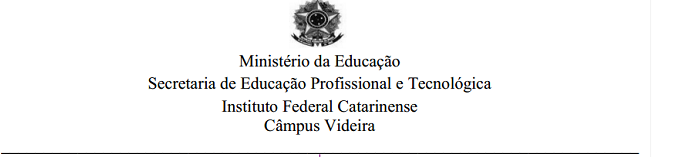
\includegraphics{images/logo.png}
		\end{center}
	\end{figure}
	%{\ABNTEXchapterfont\large{\textbf{BACHARELADO EM CIÊNCIA DA COMPUTAÇÃO}}}
	\begin{center}
		{\ABNTEXchapterfont\large\imprimirautor}
		
		\vspace*{\fill}\vspace*{\fill}
		\begin{center}
			\ABNTEXchapterfont\bfseries\Large\imprimirtitulo
		\end{center}
		\vspace*{\fill}
	\end{center}
	
	Este Trabalho de Conclusão de Curso foi julgado adequado para a obtenção do título de Nome do Título em Nome do Curso, Área de Concentração e aprovada em sua forma final pelo Curso de Nome do Curso
	
	\assinatura{\textbf{\imprimirorientador} \\ Orientador} 
	\assinatura{\textbf{Nome do Professor I} \\ Professor Convidado I}
	\assinatura{\textbf{Nome do Professor II} \\ Professor Convidado II}
	
	\begin{center}
		\vspace*{0.5cm}
		{\large\imprimirlocal}
		\par
		{\large\imprimirdata}
		\vspace*{1cm}
	\end{center}	
\end{folhadeaprovacao}
\end{comment}

\begin{folhadeaprovacao}

  \begin{center}
  \vspace*{-1.2cm}
    {\large\imprimirautor}

    \vspace*{\fill}\vspace*{\fill}\vspace*{\fill}
    {\large\imprimirtitulo}
    \vspace*{\fill}\vspace*{\fill}
    
    \hspace{.45\textwidth}
    \begin{minipage}{.5\textwidth}
        \imprimirpreambulo
    \end{minipage}%
    \vspace*{\fill}
   \end{center}
    
  \begin{center}
  	 Local (SC), Dia, Mês e Ano (data da defesa) 
  \end{center}
  

    \vspace{-1cm}

  
   \assinatura{\begin{center}\vspace{-0.6cm}\imprimirorientador \\ 
   					   Nome da Instituição
   					   \end{center}
   					    
   } 
    \begin{center}
  	\textbf{ BANCA EXAMINADORA}
   \end{center}
   \vspace{-1cm}
   \assinatura{\begin{center}\vspace{-0.6cm} Professor \\ 
      					   Nome da Instituição
   					     \end{center}
   }
    \assinatura{\begin{center}\vspace{-0.6cm}Professor \\ 
       					   Nome da Instituição
   					    \end{center}
    }
    

    \vspace*{1cm}
  
\end{folhadeaprovacao}

\setlength{\absparsep}{18pt} % ajusta o espaçamento dos parágrafos do resumo
\begin{resumo} 


O texto do resumo deve ser digitado, em um único bloco, sem espaço de parágrafo. O resumo deve ser significativo, composto de uma sequência de frases concisas, afirmativas e não de uma enumeração de tópicos. Não deve conter citações. Deve usar o verbo na voz passiva. Abaixo do resumo, deve-se informar as palavras-chave (palavras ou expressões significativas retiradas do texto) ou, termos retirados de thesaurus da área. 

\textbf{Palavras-chaves}: Palavra. Palavra. Palavra. Palavra. Palavra. 
\end{resumo}

\begin{resumo}[Abstract]
 \begin{otherlanguage*}{english}   

Elemento obrigatório somente para dissertações e tese. Resumo traduzido para outros idiomas, neste caso, inglês. Segue o formato do resumo feito na língua vernácula. As palavras-chave traduzidas, versão em língua estrangeira, são colocadas abaixo do texto precedidas pela expressão “Keywords”, separadas por ponto.
  
  \textbf{key-words}: Keyword. Keyword.Keyword.Keyword.Keyword
 \end{otherlanguage*}
\end{resumo}

\pdfbookmark[0]{\listfigurename}{lof}
\listoffigures*
\cleardoublepage

\begin{siglas}

	\item[ABNT]{Associação Brasileira de Normas Técnicas}
   \item[IBGE]{Instituto Brasileiro de Geografia e Estatística} 

\end{siglas}
% ---
% inserir o sumario
% ---
\pdfbookmark[0]{\contentsname}{toc}
\tableofcontents*
\textual

\chapter{INTRODUÇÃO}

As orientações aqui apresentadas são baseadas em um conjunto de normas elaboradas pela ABNT. Além das normas técnicas a Biblioteca também elaborou  um guia para elaboração de trabalhos acadêmicos que está disponível na sua Homepage. < http://biblioteca.ifc.edu.br/normalizacao-de-trabalhos//>. 

\section{Objetivos}

\subsection{Objetivo Geral}
	
Descrição...

\subsection{Objetivos Específicos} 

Descrição...

% 
%--------- FIM INTRODUÇÃO------------
%
\cleardoublepage

\chapter{DESENVOLVIMENTO}

\section{Exposição do Tema ou Matéria}

É a parte principal e mais extensa do trabalho detalhando o estudo ou a pesquisa realizada Deve apresentar a fundamentação teórica, a metodologia, os resultados e a discussão. Divide-se em seções e subseções conforme a NBR 6024. Quanto a sua estrutura, segue as recomendações da norma para preparação de trabalhos acadêmicos, a NBR 14724 de 2011. \cite{ABNT} 
Abaixo é apresentada a Figura 1 onde se pode visualizar a estrutura geral do trabalho acadêmico.

\begin{figure}[htb]
	\caption{\label{ciclo}Ranking de países com maior número de acesso\hspace{10cm}}
	
	\begin{center}
		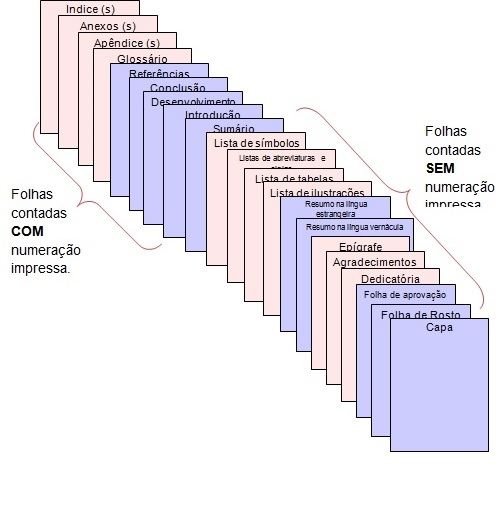
\includegraphics[scale=0.8]{images/Fig1.jpg}
	\end{center}
	\hspace{5.5cm}{Fonte: Elaboração das Autoras,2014}
\end{figure}

\section{Apresentação Gráfica do Trabalho Acadêmico}

A apresentação gráfica é a definição de tipo de fonte, margens, espaçamento, tipo de papel, etc.

\subsection{Formato (tipo de papel, tamanho da fonte, margens)}

A apresentação gráfica do TC deve seguir os seguintes requisitos:
a) utilizar papel branco ou reciclado, formato A4 (21,0 x 29,7 cm);
b) utilizar o anverso da folha para os elementos pré-textuais;
c) poderá ser utilizado o anverso e verso da folha para impressão dos elementos 
    textuais e pós-textuais;
c) digitar o texto na cor preta;
d) fonte tamanho 12 para o texto;
e) fonte tamanho 10 para citações longas, notas de rodapé, legendas e fontes 
    (identificação) das ilustrações e tabelas e paginação;
f) optar por fontes arredondadas (Times New Roman ou Arial);
g) adotar as margens:
    - para o anverso da folha:
       - superior de 3 cm, 
       - inferior de 2 cm,
       - esquerda de 3 cm,
       - direita de 2 cm,
     - para o verso:
        - superior de 3 cm, 
        - inferior de 2 cm,
        - esquerda de 2 cm,
       - direita de 3 cm,
h) primeira linha do parágrafo com recuo de 2 cm a partir da margem esquerda;
          i) citação longa (com mais de três linhas) com recuo de 4 cm a partir da margem
    esquerda;
j) nota de rodapé digitada dentro das margens indicadas, devendo ficar separada do 
   texto por um traço de 5 cm a partir da margem esquerda.

\subsection{Espaçamento}

O espaçamento que você deve adotar na formatação é:
a) espaço 1,5  - todo o texto,
          b) um espaço de 1,5;
     - separa o texto da citação longa,
     - separa cada título das seções e subseções do texto que os precedem e que os 
       sucedem,
c) espaço simples para;
    - citações longas,
    - notas de rodapé,
    - referências,
    - legenda e fonte das ilustrações e tabelas,
    - natureza do trabalho.
e) um espaço simples -  entre uma referência e outra, na lista de referências ao final do trabalho.

\subsection{Indicativo de seção e numeração progressiva}

Seção é a divisão do TC, aplicada somente aos elementos textuais e visa expor numa sequência lógica o relacionamento da matéria e a permitir a sua localização. De acordo com a NBR 6024 as seções também podem ser subdividas em subseções.
A seção primária é a principal divisão do texto do TC, que sempre deverá ser grafada em números inteiros a partir do 1, alinhados à esquerda por um espaço de caractere e iniciar em página distinta e ímpar (anverso). As demais são chamadas de subseções e/ou seções secundária, terciária, quaternária e quinária. Se for necessário enumerar os diversos assuntos de uma seção que não possua título, esta deve ser subdividida em alíneas. As alíneas são ordenadas alfabeticamente e terminam em ponto e vírgula, exceto a última que termina em ponto. Todas as seções devem conter um texto relacionado a elas (FIGURA 2) .
Exemplo sugerido pelo IFC:
1 SEÇÃO PRIMÁRIA (maiúsculas em negrito)
1.1 SEÇÃO SECUNDÁRIA (maiúsculas)
1.1.1 Seção terciária (em negrito com primeira letra maiúscula)
1.1.1.1 Seção quaternária (primeira letra maiúscula)
1.1.1.1.1 Seção quinária (em itálico com primeira letra maiúscula)
a) alínea (primeira letra minúscula);
b) alínea;
    - subalínea.
c) alínea.
2 SEÇÃO PRIMÁRIA 
2.1 SEÇÃO SECUNDÁRIA 
2.1.1 Seção terciária 
.
.
.
\begin{figure}[htb]
	\caption{\label{ciclo}Ranking de países com maior número de acesso\hspace{10cm}}
	
	\begin{center}
		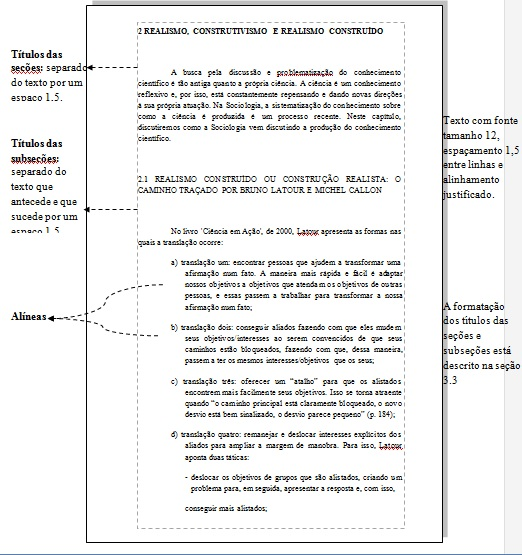
\includegraphics[scale=1.1]{images/Fig2.jpg}
	\end{center}
	\hspace{5.5cm}{Fonte: Elaboração das Autoras,2014}
\end{figure}

\subsection{Paginação}

Para o TC, as páginas pré-textuais devem ser contadas, mas não numeradas. A contagem será a partir da folha de rosto. A numeração deve configurar a partir da primeira folha textual em algarismos arábicos e sendo sequencial até o final do trabalho. 
A paginação da(s) referência(s), do(s) anexo(s) e do(s) apêndice(s) deve ser numerada sequencialmente no TC. As páginas que não permitem a inclusão de números também são contadas (mapas, documentos, ilustrações, etc.).
O número da página deve aparecer no canto superior direito da folha, a 2 cm da borda superior, ficando o último algarismo a 2 cm da borda direita da folha.
Para trabalhos com mais de um volume, a numeração sequencial das folhas deve ser mantida. Se o trabalho contiver apêndice e anexo, a numeração das páginas deve dar sequência ao texto principal.

\subsection{Lombada}

A lombada é um elemento opcional para o TC e na sua estrutura, deve conter os seguintes elementos: 
a)	nome(s) do(s) autores, quando houver;
b)	título;
c)	identificação do volume, fascículo e data, se houver.
Todos os elementos que compõem a lombada devem ser centralizados em suas áreas, com fonte tamanho 12, espaçamento simples e todas as letras maiúsculas (FIGURA 3).

\begin{figure}[htb]
	\caption{\label{ciclo}Ranking de países com maior número de acesso\hspace{10cm}}
	
	\begin{center}
		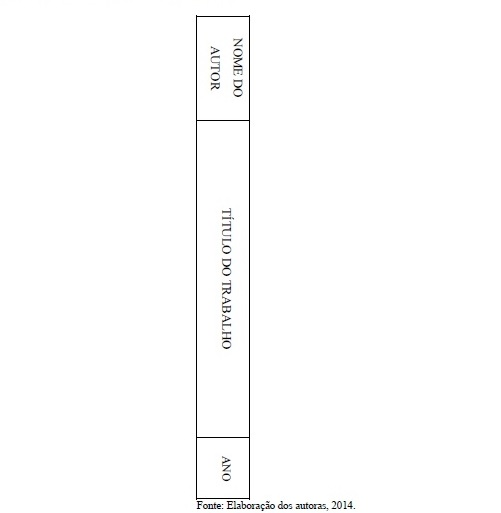
\includegraphics[scale=1.1]{images/Fig3.jpg}
	\end{center}
\end{figure}

% 
%--------- FIM DESENVOLVIMENTO------------
%
\cleardoublepage

\chapter{CONCLUSÃO}

As conclusões devem responder às questões da pesquisa, em relação aos objetivos e hipóteses. Devem ser breves podendo apresentar recomendações e sugestões para trabalhos futuros.  
\postextual
\bibliography{referencias}
\end{document}








